\documentclass[12pt, a4paper]{article} 
\usepackage{amsmath,amsfonts,amssymb,amsthm,mathtools}
\usepackage{fontspec}       
\setmainfont{Roboto}      

\usepackage{unicode-math}   
\setmathfont{Asana Math}      
\usepackage{polyglossia}       
\setdefaultlanguage{russian} 
\setotherlanguage{english}

\ifx\pdfoutput\undefined
\usepackage{graphicx}
\else
\usepackage[pdftex]{graphicx}
\fi


\begin{document}
\textbf{\centerline{ДОМАШНЯЯ РАБОТА №1}
\centerline{Подготовила Ивлева Анастасия} }
\section{Факты о моей личности:}

\begin{itemize}
 \item Обожаю милых и пушистых животных, они так радают и успокаивают;
 \item Семья и близкие - самое главное;
 \item Вдохновляет природа: леса, реки, озера, особенно горы!;
 \item В моей семье все родились 20го числа каждого месяца осени;
 \item Во мне заложен избыток доброты;
 \item Люблю лежать звездочкой в море и наслаждаться видом гор;
 \item Ну вот прямо очень сильно мнительная;
 \item Не люблю смотреть ужасы, потому что вроде и не верю в них, но вроде и страшно;
 \item Очень прямолинейна;
 \item Очень нравится фильм "Крестный отец".
\end{itemize}

\section{Моя фотография}
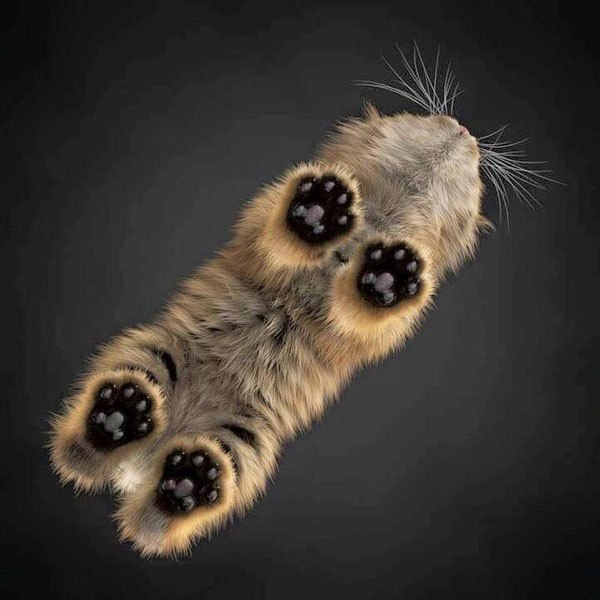
\includegraphics[width=15 cm]{image.jpg}

\section{Любимые сложные формулы}

\begin{equation*}
\begin{aligned}
Flow_{i,t+1} &= \sum_{\substack{k}} γ_k Agek_{it} fr_{it}-r_{mt})+
\sum_{k} δ_k Agek_{it} +α_1(r_{it-1}-rm_{t-1})+\\
  &+ α_2(r_{it-2}-rm_{t-2}) + α_3((r_{it+1}-rm_{t+1}) +\\
  &+ α_4IndustryGrowth_{t+1}+α_5log(Assets_{it})+ ε_{it+1} 
\end{aligned} \tag{æ} 
\end{equation*}

\begin{equation*}
{\int\int}_{D}f(x,y)dxdy = \int_{a}^{b} dx \int_{c}^{d}f(x,y)dy
\tag{ææ} 
\end{equation*}

\begin{equation*}
\lim_{x \to \{x_o} (f(x))^{g(x)} = e^{\lim\limits_{x \to\ 0}\frac{ln(f(x))}{\frac{1}{g(x)}}}
% филипп, не удалось заставить его работать со скобкой, которая слева ({x_o})
\tag{æææ}
\end{equation*}




\begin{equation} 
\begin{aligned} 
&AB = \begin{pmatrix}
a_{11} & \dots & a_{1n} \\
\vdots & \ddots & \vdots \\
a_{m1} & \dots & a_{mn}
\end{pmatrix}
\begin{pmatrix}
b_{11} & \dots & b_{1n} \\
\vdots & \ddots & \vdots \\
b_{m1} & \dots & b_{mn}
\end{pmatrix} = \\
&=\begin{pmatrix}
{a_{11}b_{11}+a_{12}b_{21}+\dots+a_{1n}b_{n1}} & \dots & {a_{11}b_{1q}+a_{12}b_{2q}+\dots+a_{1n}b_{nq}} \\
\vdots & \ddots & \vdots \\
{a_{p1}b_{11}+a_{p2}b_{21}+\dots +a_{pn}b_{n1}} & \dots & {a_{p1}b_{1q}+a_{p2}b_{2q}+\dots +a_{pn}b_{nq}}

\end{pmatrix}
\end{aligned} \tag{ææææ} 
\end{equation}

\begin{equation}
JB=n\left(\frac{s^2}{6}+\frac{(k-3)^2}{24}\right)
\tag{æææææ}
\end{equation}


\begin{enumerate}
 \item Формулу \ref{æ} я так сильно люблю, потому что несколько недель я пыталась понять ее и найти для нее данные, но позже оказалось, что она мне вовсе не нужна для того, чтобы считать чистый денежный поток года t+1!
 \item Что касается \ref{ææ}, какие же мы математики, если не любим эту формулу!?
 \item Обращаясь к формуле \ref{æææ}, на первом курсе мне очень нравилась эту формула, потому что позволяет быстро решать некоторые интегралы показательной степени, к тому же я смогла ее быстро запомнить.
 \item А что говорить об этой \ref{ææææ}, вот уже третий год она не покидает нас :)
 \item До сих не совсем понимаю суть такого теста, как Харке-Бера под номером \ref{æææææ}

\end{enumerate}

\subsection{Ненавистная формула :)}
Думаю, что многим эта формула разбила сердце, я тому не исключение!

\[\hat\sigma_{\hat\beta_1} = \frac{1}{n} \frac{\frac{1}{n-2}\sum_{i=1}^n(x_i-{\bar x})^2 {\hat\{u_i^2}}{(\frac{1}{n}\sum_{i=1}^n(x_i-{\bar x})^2)^2}\]


\end{document}


